\documentclass[border=5pt]{standalone}

\usepackage[T1]{fontenc}
\usepackage{garamondx}
\usepackage[garamondx,cmbraces]{newtxmath}

\usepackage{standalone}
\usepackage{tikz}
    \usetikzlibrary{arrows,shapes,positioning}

\definecolor{blue}{HTML}{0072B2}
\definecolor{pink}{HTML}{CC79A7}

\begin{document}

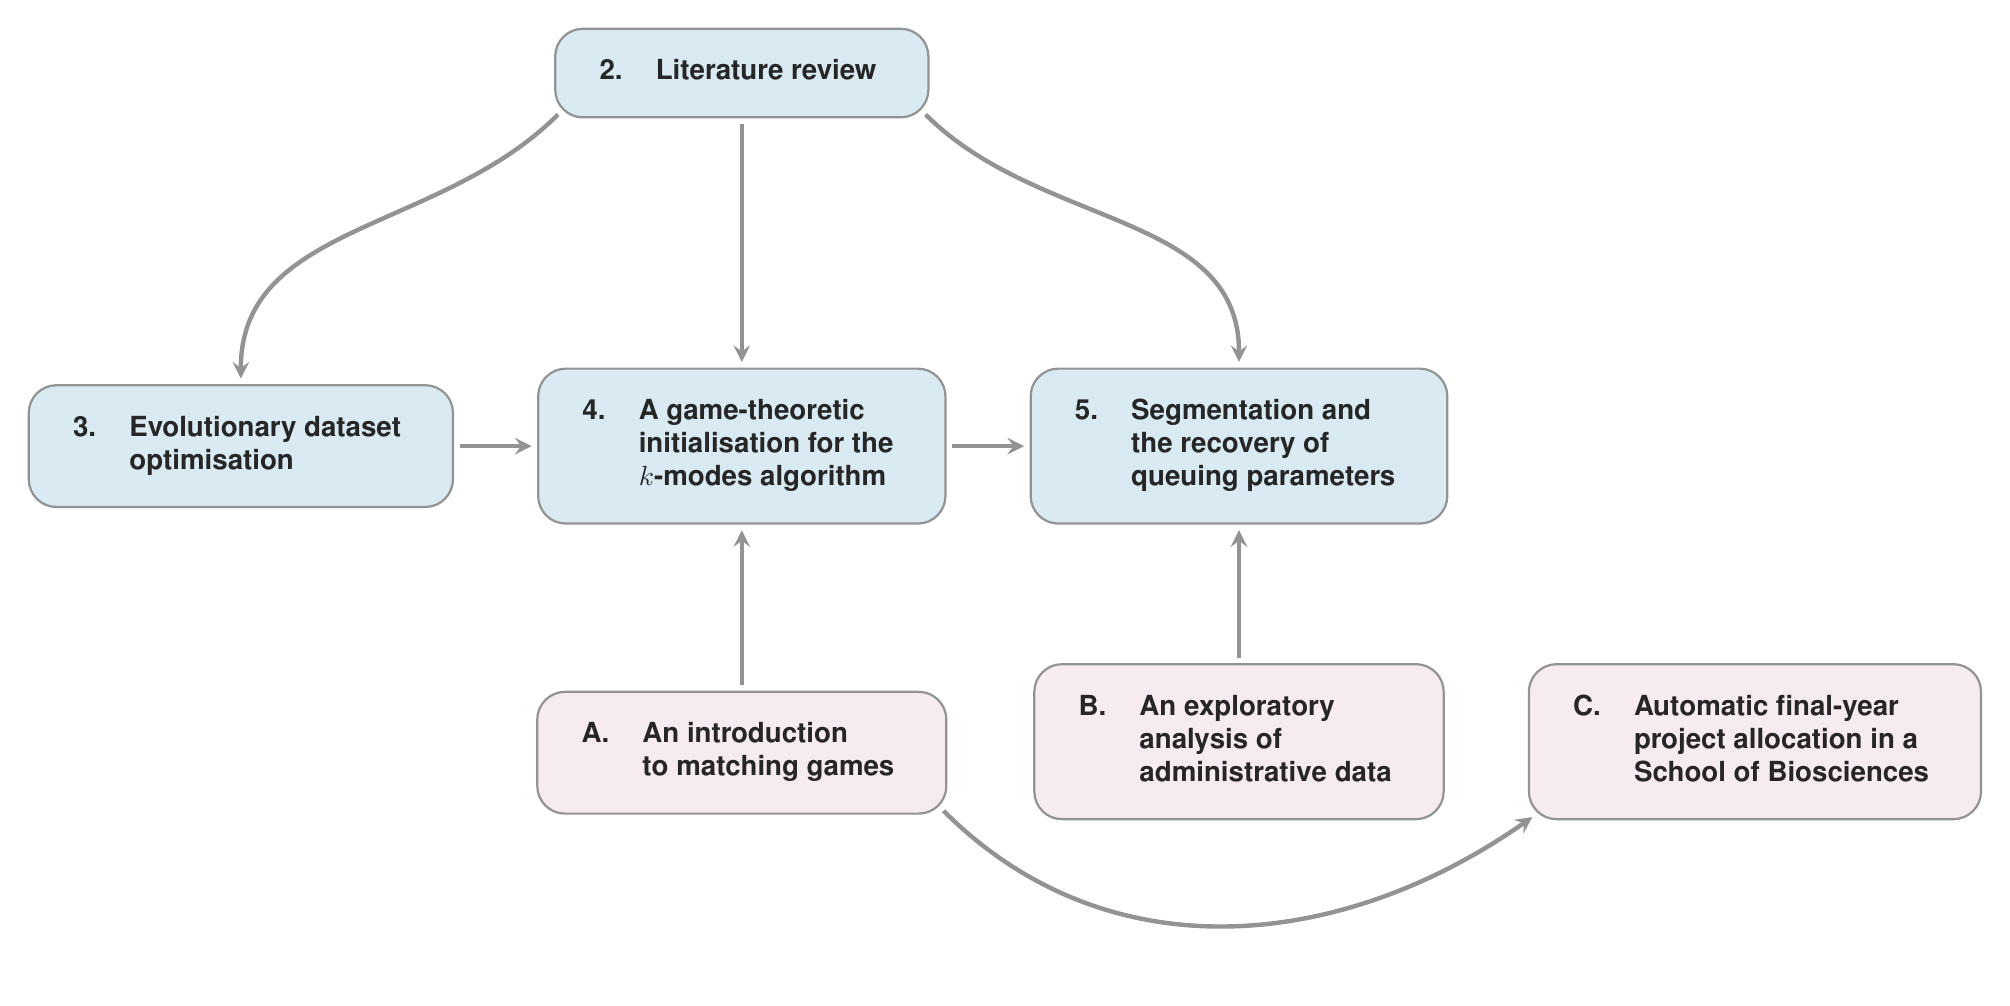
\begin{tikzpicture}

    %% Style settings
    \usefont{T1}{phv}{b}{n}\color{black!85}\selectfont
    \tikzstyle{chapter} = [%
        inner sep=1em,
        rounded corners=1em,
        draw=gray!85,
        thick,
        fill=blue!15,
        minimum height=3em,
    ]
    \tikzstyle{appendix} = [chapter, fill=pink!15]
    \tikzstyle{connection} = [%
        -stealth,
        ultra thick,
        shorten <=2pt,
        shorten >=2pt,
        gray!85,
    ]

    %% Nodes
    \node[chapter] (lit) {%
        \textbf{%
            \begin{tabular}{ll}
                2. & Literature review
            \end{tabular}
        }
    };

    \node[below=9em of lit, chapter] (kmodes)
        {%
            \textbf{%
                \begin{tabular}{ll}
                    4. & A game-theoretic\\
                       & initialisation for the\\
                       & \(k\)-modes algorithm
                \end{tabular}
            }
        };

    \node[left=3em of kmodes, chapter] (edo)
        {%
            \textbf{%
                \begin{tabular}{ll}
                    3. & Evolutionary dataset\\
                       & optimisation
                \end{tabular}
            }
        };

    \node[right=3em of kmodes, chapter] (copd)
        {%
            \textbf{%
                \begin{tabular}{ll}
                    5. & Segmentation and\\ 
                       & the recovery of\\
                       & queuing parameters
                \end{tabular}
            }
        };

    \node[below=6em of kmodes, appendix] (matching)
        {%
            \textbf{%
                \begin{tabular}{ll}
                    A. & An introduction\\
                       & to matching games
                \end{tabular}
            }
        };

    \node[below=5em of copd, appendix] (data)
        {%
            \textbf{%
                \begin{tabular}{ll}
                    B. & An exploratory\\
                       & analysis of\\
                       & administrative data
                \end{tabular}
            }
        };

    \node[right=3em of data, appendix] (biosi)
        {%
            \textbf{%
                \begin{tabular}{ll}
                    C. & Automatic final-year\\
                       & project allocation in a\\
                       & School of Biosciences
                \end{tabular}
            }
        };

    %% Arrows
    \draw[connection, shorten <=-2pt]
        (lit.south west) to[out=225,in=90] (edo.north);
    
    \draw[connection] (lit.south) to[out=270,in=90] (kmodes.north);
    
    \draw[connection, shorten <=-2pt]
        (lit.south east) to[out=315, in=90] (copd.north);

    \draw[connection] (edo.east) to (kmodes.west);
    
    \draw[connection] (kmodes.east) to (copd.west);

    \draw[connection] (matching.north) to (kmodes.south);

    \draw[connection] (data.north) to (copd.south);

    \draw[connection, shorten <=-2pt, shorten >=-2pt]
        (matching.south east) to[out=315, in=215] (biosi.south west);

\end{tikzpicture}

\end{document}
